%%%%%%%%%%%%%%%%%%%%%%%%%%%%%%%%%%%%%%%%%
% fphw Assignment
% LaTeX Template
% Version 1.0 (27/04/2019)
%
% This template originates from:
% https://www.LaTeXTemplates.com
%
% Authors:
% Class by Felipe Portales-Oliva (f.portales.oliva@gmail.com) with template
% content and modifications by Vel (vel@LaTeXTemplates.com)
%
% Template (this file) License:
% CC BY-NC-SA 3.0 (http://creativecommons.org/licenses/by-nc-sa/3.0/)
%
%%%%%%%%%%%%%%%%%%%%%%%%%%%%%%%%%%%%%%%%%

%----------------------------------------------------------------------------------------
%	PACKAGES AND OTHER DOCUMENT CONFIGURATIONS
%----------------------------------------------------------------------------------------

\documentclass[
    12pt, % Default font size, values between 10pt-12pt are allowed
%letterpaper, % Uncomment for US letter paper size
%spanish, % Uncomment for Spanish
]{fphw}

% Template-specific packages
\usepackage[utf8]{inputenc} % Required for inputting international characters
\usepackage[T1]{fontenc} % Output font encoding for international characters
\usepackage{mathpazo} % Use the Palatino font

\usepackage{graphicx} % Required for including images

\usepackage{booktabs} % Required for better horizontal rules in tables

\usepackage{listings} % Required for insertion of code

\usepackage{enumerate} % To modify the enumerate environment
\usepackage{textcomp}
\usepackage{amsmath}
\usepackage{subcaption}
\usepackage[justification=centering]{caption}
\usepackage{float}
\usepackage{xcolor}
\usepackage{polski}
\usepackage[polish]{babel}
\usepackage{csvsimple}
\usepackage{mathtools}
\usepackage{ulem}
\usepackage{hyperref}
\usepackage{makecell}
\renewcommand{\cellalign}{cl}

\definecolor{codegreen}{rgb}{0,0.6,0}
\definecolor{codegray}{rgb}{0.5,0.5,0.5}
\definecolor{codepurple}{rgb}{0.58,0,0.82}
\definecolor{backcolour}{rgb}{0.95,0.95,0.92}

\lstdefinestyle{mystyle}{
    backgroundcolor=\color{backcolour},
    commentstyle=\color{codegreen},
    keywordstyle=\color{magenta},
    numberstyle=\tiny\color{codegray},
    stringstyle=\color{codepurple},
    basicstyle=\ttfamily\footnotesize,
    breakatwhitespace=false,
    breaklines=true,
    captionpos=b,
    keepspaces=true,
    numbers=left,
    numbersep=5pt,
    showspaces=false,
    showstringspaces=false,
    showtabs=false,
    tabsize=2
}

\lstset{style=mystyle}

\renewcommand{\lstlistlistingname}{Spis listingów}
%----------------------------------------------------------------------------------------
%	ASSIGNMENT INFORMATION
%----------------------------------------------------------------------------------------

\title{Projekt 2: Javascript} % Assignment title

\author{Monika Nawój} % Student name

\date{\today} % Due date

\institute{Politechnika Warszawska \\ Wydział Elektroniki i Technik Informacyjnych} % Institute or school name

\class{Zaawansowane aplikacje internetowe (2021Z)} % Course or class name

\professor{dr inż. Przemysław Korpas} % Professor or teacher in charge of the assignment

%----------------------------------------------------------------------------------------

\begin{document}

    \maketitle % Output the assignment title, created automatically using the information in the custom commands above

%----------------------------------------------------------------------------------------
%	ASSIGNMENT CONTENT
%----------------------------------------------------------------------------------------


    \section{Instrukcja}

    \subsection{Instalacja paczek}
    Aby zainstalować potrzebne paczki npm, należy uruchomić komendę \textit{npm start} w głównym folderze projektu.
    \begin{lstlisting}
            npm install
    \end{lstlisting}

    \subsection{Uruchomienie aplikacji}
    Po zainstalowaniu potrzebnych paczek, możemy uruchomić serwer z aplikacją za pomocą komendy \textit{npm start}
    również w folderze głównym projektu.
    \begin{lstlisting}
            npm start
    \end{lstlisting}
    Aplikacja nasłuchuje na porcie: \url{http://localhost:3000}.


    \section{Wybory projektowe}
    Wybranym frameworkiem front-endowym do wykonania tego projektu jest \textbf{React}.
    Główną przyczyną tego wyboru jest istniejące doświadczenie w tworzeniu
    projektów przy użyciu Reacta oraz łatwość utworzenia nowego projektu za pomocą \textbf{Create React App}.
    \\
    \textbf{Bootstrap} został wybrany jako framework CSS również ze względu na doświadczenie
    pracy z tym właśnie frameworkiem oraz ze względu na łatwość w użyciu.
    \\
    Dodatkowo została użyta biblioteka \textbf{uuid} do generowania unikatowych identyfikarów przy dodawaniu
    nowych filmów do kolekcji.


    \section{Opis kodu}
    Tabela~\ref{tab:comp} zawiera opis głównych komponentów aplikacji.
    \begin{table}[H]
        \centering
        \begin{tabular} {| l | l |}
            \hline
            Komponent   & Opis        \\
            \hline
            App         & \makecell{Jest to bazowy komponent aplikacji, dodaje komponenty niżej \\ w hierarchi do \textit{DataContextProvider}.} \\
            AddMovie    & \makecell{Komponent zawierający logikę dodawania nowego filmu do kolekcji.} \\
            \hline
            EditMovie   & \makecell{Komponent zawierający logikę edytowania wybranego filmu z listy.} \\
            \hline
            MovieForm   & \makecell{Komponent zawierający formularz z polami filmu Formularz ten jest \\ wykorzystywany zarówno w komponencie \textit{AddMovie} jak i \textit{EditMovie}. } \\
            \hline
            MovieList   & \makecell{Komponent zawierający listę dostępnych filmów wraz ze wszystkimi \\ kontrolkami.} \\
            \hline
            PriceFilter & \makecell{Komponent zawierający logikę filtrowania listy ze względu na \\ przedział \textit{od/do}}. \\
            \hline
            SortButton  & \makecell{Komponent zawierający logikę sortownia na wybranych kolumnach. \\  Został wykorzystany dla kolumny \textit{Tytuł} oraz \textit{Cena}.} \\
            \hline
            DataContextProvider & \makecell{Komponent dostarczający \textit{context} aplikacji do reszty kompoentów. \\
            \textit{DataContext} zawiera stan aplikacji z listą dostępnych filmów \\ oraz dodatkowych pól i metod modyfikujących ten stan.} \\
            \hline
        \end{tabular}
        \caption{Główne komponenty aplikacji}
        \label{tab:comp}
    \end{table}


    \section{Przykładowe zrzuty ekranu}
    \begin{figure}[H]
        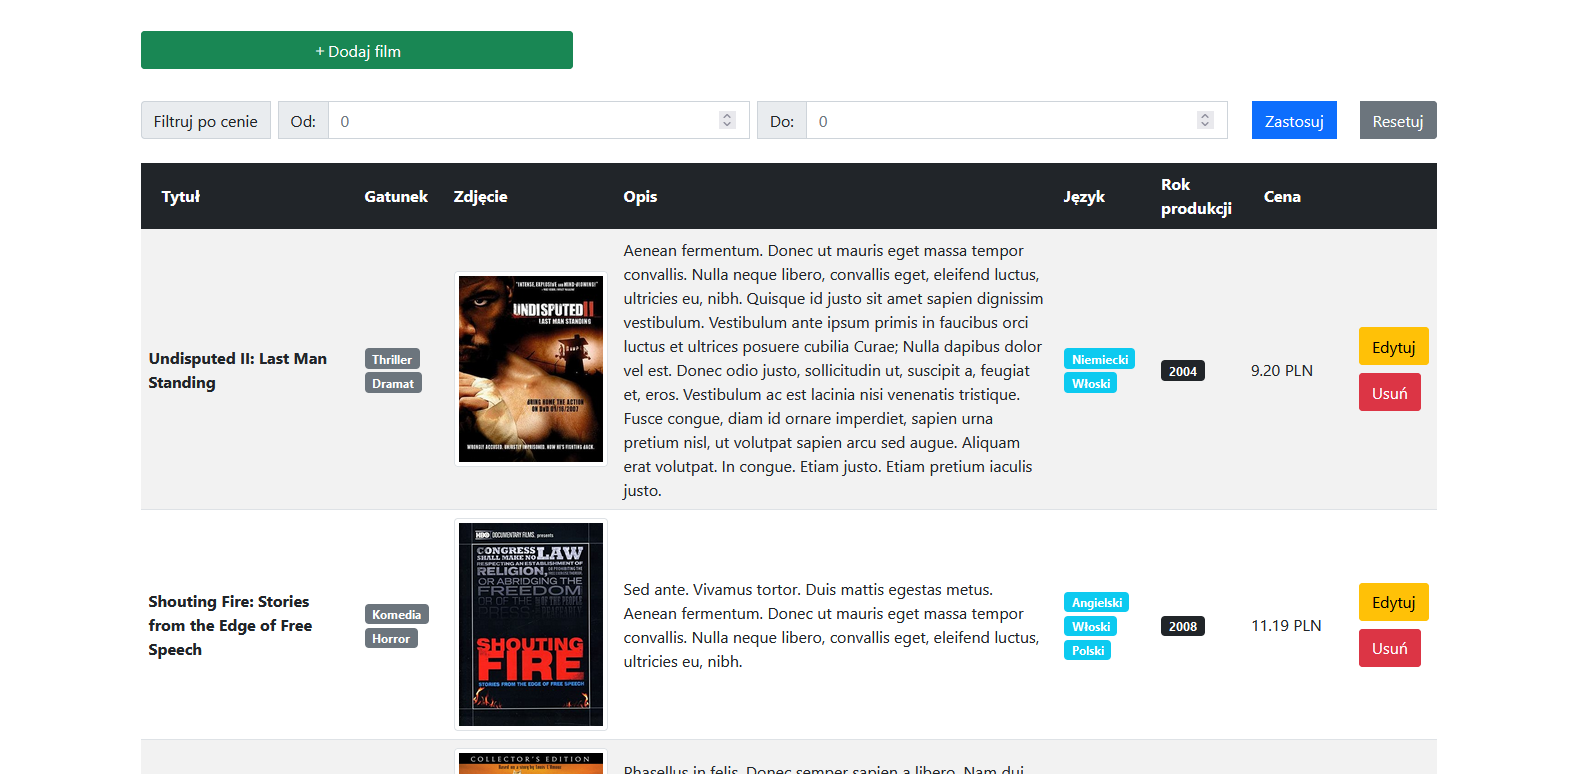
\includegraphics[width=\linewidth]{./assets/1.PNG}
        \caption{Lista filmów}
        \label{fig:movie-list}
    \end{figure}

    Rysunek~\ref{fig:movie-list} przedstawia główny widok aplikacji - listę filmów, zawierającą tytuł,
    gatuek, zdjęcie okładki, króki opis, dostępne wersje językowe filmu, rok produkcji,
    cena filmu oraz przyciski edycji poszczególnych wierszy.
    Lista może być sortowana po kolumnie tytułu lub ceny.
    Dodatkowo dostępne są filtry przedziału \textit{od/do} dla ceny.

    \begin{figure}[H]
        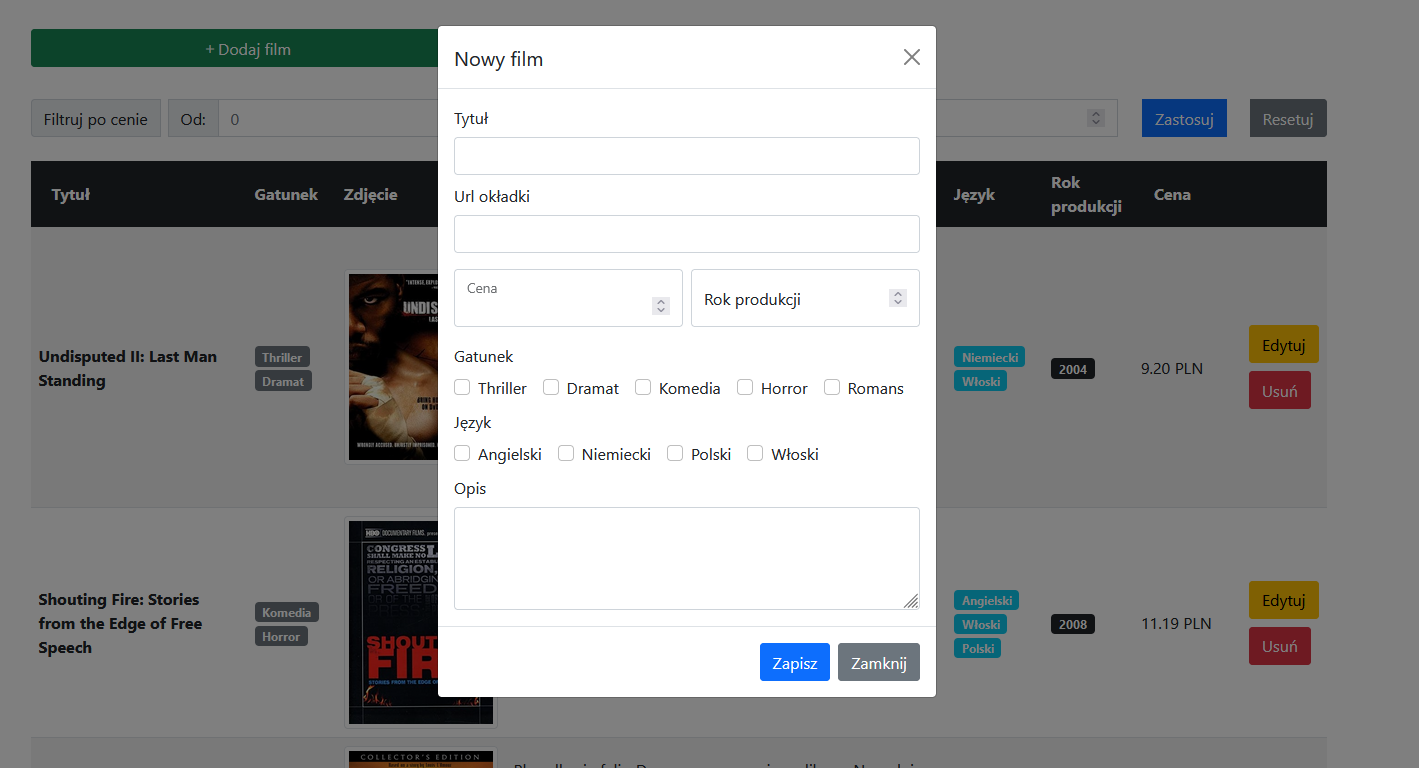
\includegraphics[width=\linewidth]{./assets/2.PNG}
        \caption{Dodawanie nowego filmu}
        \label{fig:add}
    \end{figure}

    Rysunek~\ref{fig:add} przedstawia modal dodawania filmu do kolekcji, który pojawia się po naciśnięciu przycisku
    \textit{Dodaj film}.

    \begin{figure}[H]
        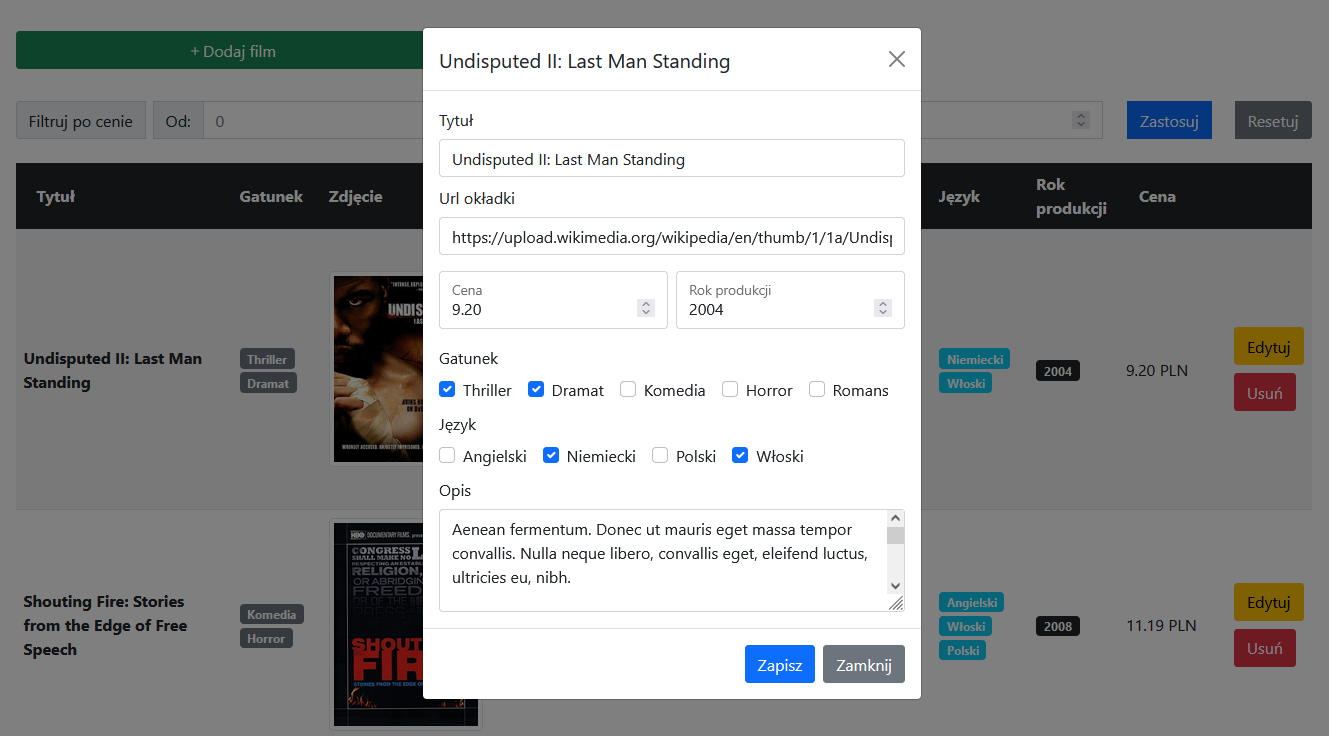
\includegraphics[width=\linewidth]{./assets/3.PNG}
        \caption{Edycja filmu}
        \label{fig:edit}
    \end{figure}

    Rysunek~\ref{fig:edit} przedstawia analogiczny modal do edycji wybranego filmu.

    \newpage
    \listoffigures
    \listoftables

\end{document}
